%% progress-report-8-SubmapVisualization+ROSPackage tex file.
%% Completed By Yuyang Rong(rongyy@shanghaitech.edu.cn) and
%% Jianxiong Cai(caijx@shanghaitech.edu.cn)
%%
%% To edit this file, please use indentions with tab size of 2.
%%

%% File name unchanged. This is just a temp file.

\documentclass[conference,compsoc]{IEEEtran}
\usepackage{cite}
\usepackage{listings}
\usepackage{blindtext}
\usepackage{enumitem}
% for coding highlight
\usepackage{graphicx}
\usepackage{subfigure}
\usepackage[colorlinks=true,urlcolor=blue]{hyperref}
\usepackage{amsmath, amsthm, amssymb}
\usepackage{subfloat}
\usepackage{ulem}
\usepackage{float}
\usepackage{indentfirst}
\newcommand{\subparagraph}{}
\begin{document}
\title{
	Computer Vision Course Project Milestone Report\\
	Gambody \\
}


% author names and affiliations
% use a multiple column layout for up to three different
% affiliations
\author{
	\IEEEauthorblockN{Yuyang Rong, Jingyi Huang, Anqi Pang, Jianxiong Cai, Ziyue Li}
	\IEEEauthorblockA{
		School of Information Science and Technology \\
		ShanghaiTech University \\
	}
}

\maketitle

\begin{abstract}
	In this milestone report we are going to propose the problems we want to solve aiming at our goal of implementing the visual game Gambody. We will clarify the technical approach we are using at present and what we have achieved so far. The remaining milestones including the dates and sub-goals will be given furthermore.
\end{abstract}
\section{Introduction}
	\par
		We found a popular game called \textit{Hole in the Wall}. In this game one (or two) player(s) are facing a moving wall with a certain shape of hole, the player have to make certain pose to pass the moving wall or he will be pushed into the water.
		Such game is interesting but householders can never have the privilege to play in family gatherings or parties since one can hardly find a moving wall nor adequate safety measurements.
		\begin{figure}[h]
			\centering
			
\includegraphics[width=0.8\linewidth]{./Pic/HIW_Logo}
			\caption{Game Logo}
		\end{figure}
		\begin{figure}[h]
			\centering
			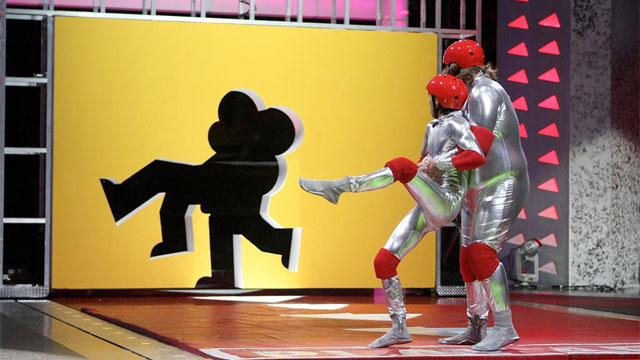
\includegraphics[width=0.45\linewidth]{./Pic/HIW_RedTeam}
			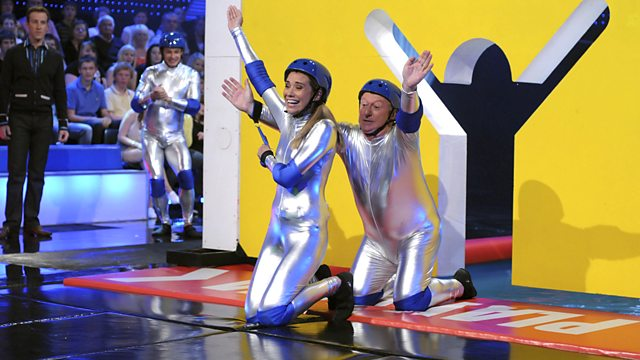
\includegraphics[width=0.45\linewidth]{./Pic/HIW_BlueTeam}
			\caption{Two players in the game posing to pass the wall.}
		\end{figure}
	\par

	\par
		To fix this, we are going to implement a system based on camera so that every one can play this game.
		In our work, we will be using camera to track real person, it will also give player a bounding box (moving wall).
		The box and player's outfit is compared by our system, the return should be a pass (True) or no pass (False).
\section{Technical Approach}

\section{Milestones Achieved So Far}

\section{Remaining Milestones}


% \bibliographystyle{IEEEtran}
% %% De-comment this line if you have any reference.
% %% And don't forget to change .bib file.
% \bibliography{milestone}
\end{document}
